\chapter{پیشینه پژوهش}

\section{مقدمه}
ظهور مدل‌های Transformer و انقلاب در یادگیری عمیق، یکی از تحولات اساسی در حوزه پردازش زبان طبیعی (NLP) و یادگیری ماشین به شمار می‌رود. این مدل‌ها باعث تغییرات عمده‌ای در نحوه ساخت و آموزش مدل‌های زبانی و همچنین در بسیاری از کاربردهای دیگر یادگیری ماشین شده‌اند. و توانستند بسیاری از مشکلات مدل های قبلی را حل کنند.

\section{مشکلات ترجمه ماشینی و ترانسفورمرها:}
در ابتدا، ترجمه ماشینی (MT) یک چالش اساسی در زمینه پردازش زبان طبیعی بود. مدل‌های اولیه‌ای مانند مدل‌های مبتنی بر قواعد (Rule-based models) برای ترجمه استفاده می‌شدند که در آن‌ها، ترجمه‌ها به صورت دستی با استفاده از قواعد زبانی مشخص تنظیم می‌شدند.
این روش‌ها هرچند دقیق بودند، اما محدودیت‌های زیادی داشتند و نمی‌توانستند ویژگی‌های پیچیده‌تر زبان را مدل‌سازی کنند.
سپس مدل‌های آماری (Statistical Models) معرفی شدند. این مدل‌ها از داده‌های ترجمه‌شده برای آموزش مدل‌های آماری استفاده می‌کردند که احتمال ترجمه‌ای صحیح را براساس شواهد آماری محاسبه می‌کردند. مدل‌هایی مانند مدل‌های ترجمه آماری مبتنی بر جمله (Phrase-based Statistical Models) از این نوع بودند، که قادر به ترجمه جملات بهتر از مدل‌های مبتنی بر قواعد بودند، اما هنوز هم در ترجمه‌های پیچیده با مشکلاتی روبه‌رو بودند.  بعد از این مدل ها مدل ها بازگشتی به وحود آمدند که مشکلات آن را در فصل گذشته بیان کردیم و د نهایت این مشکلات باعث به وجود آمدن ترانسفورمر ها شد.

\section{ظهور ترانسفورمر ها:}
در سال 2017 مقاله ... توسط گوگل منتشر شد که مفهوم جدیدی به نام ترانسفورمر ها را بیان کرد.
این مقاله به موضوع ترجمه ماشینی پرداخت و نشان داده با استفاده از مفهوم مکانیزم توجه (Attention-Mechanism) می توان بسیاری از مشکلات مدل های قبلی را حل کرد.
این مدل ها از پردازش موازی استفاده میکردند بر خلاف مدل های قبلی که از پردازش های سریالی استفاده میکردند. و این مدل ها قادر هستند به طور همزمان به تمام بخش های ورودی توجه کند.
و این کار باعث شد که ترانسفورمر ها در پردازش تصویر و متن بسیار سریع تر و دقیق تر از مدل های قبلی عمل کنند.


 \section{معماری ترانسفورمر ها:}
 
 در تصویر ... معماری ترانسفورمر نمایش داده شده است  و بخش هاو اجزای مختلف آن مشخص شده است که از دو بخش اصلی انکودر و دیکدر تشکیل شده است هدف انکودر این است که داده ورودی را میگیرد  و ویژگی های آن را استخراج میکند و هدف دیکدر این است که ویژگی های استخراج شده را به زبان مقصد تبدیل میکند. که به طور مختصر به معماری  و بخش های مختلف آن میپردازیم.
 
 \begin{figure}[h]
 	\centering
 	\begin{minipage}[b]{0.45\textwidth}
 		\centering
 		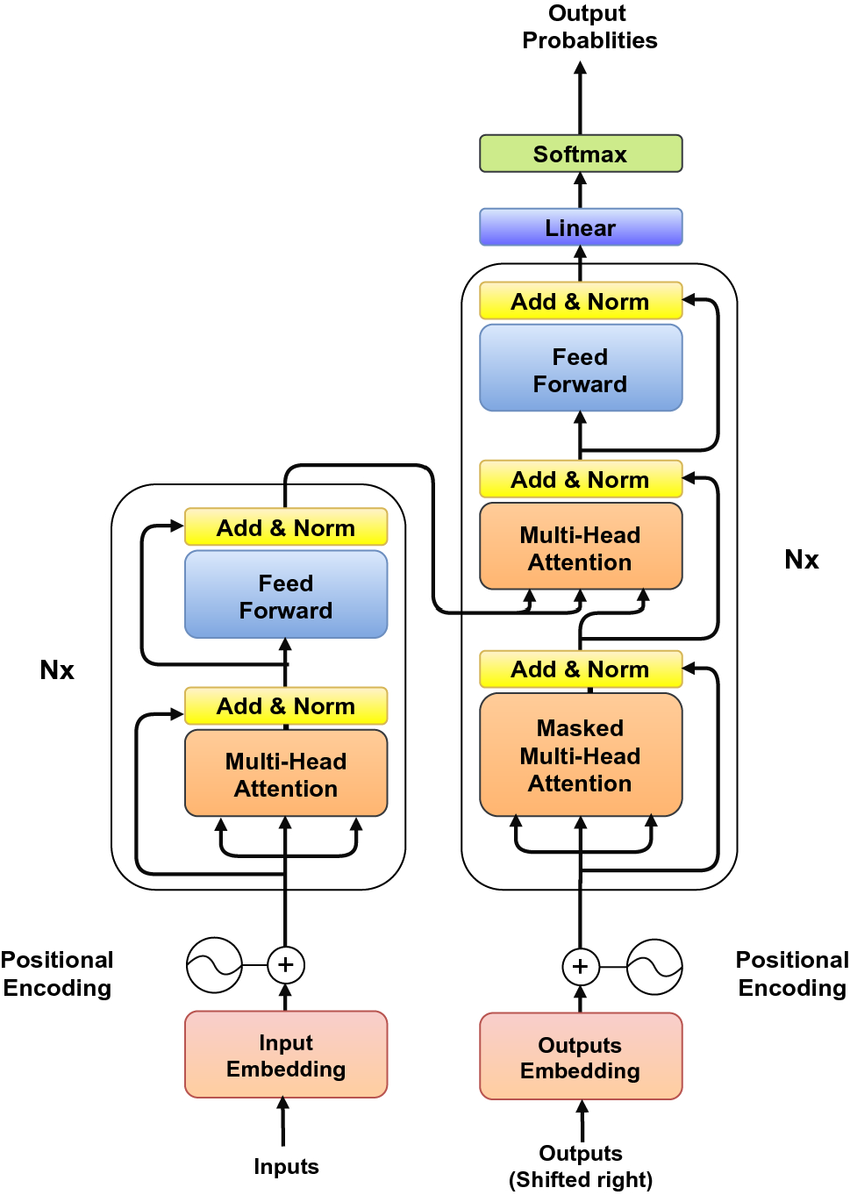
\includegraphics[width=\textwidth]{Transformer-model-architecture.png}
 		\caption{معماری ترانسفورمر ها}
 		\label{fig:transformer_architecture}
 	\end{minipage}
 	\hfill

 \end{figure}

\subsection{Embedding:}
در زبان طبیعی کلمات به شکل رشته های متنی هستند مانند کتاب ، ماشین و ... 
کامپیوتر ها نمیتوانند به طور مستقیم به شکل رشته های متنی این کلمات را پردازش کنند. 
به همین دلیل در یادگیری ماشین ما این کلمات را به شکل یک بردار نمایش می دهیم. و آن بردار بیانگر آن کلمه در مدل است تا ماشین بتواند آن کلمه را پردازش کند.

این بردار ها ویژگی های کلمه را فضای عددی نمایش میدهد. 





